\documentclass[11pt,preprint, authoryear]{elsarticle}

\usepackage{lmodern}
%%%% My spacing
\usepackage{setspace}
\setstretch{1.2}
\DeclareMathSizes{12}{14}{10}{10}

% Wrap around which gives all figures included the [H] command, or places it "here". This can be tedious to code in Rmarkdown.
\usepackage{float}
\let\origfigure\figure
\let\endorigfigure\endfigure
\renewenvironment{figure}[1][2] {
    \expandafter\origfigure\expandafter[H]
} {
    \endorigfigure
}

\let\origtable\table
\let\endorigtable\endtable
\renewenvironment{table}[1][2] {
    \expandafter\origtable\expandafter[H]
} {
    \endorigtable
}


\usepackage{ifxetex,ifluatex}
\usepackage{fixltx2e} % provides \textsubscript
\ifnum 0\ifxetex 1\fi\ifluatex 1\fi=0 % if pdftex
  \usepackage[T1]{fontenc}
  \usepackage[utf8]{inputenc}
\else % if luatex or xelatex
  \ifxetex
    \usepackage{mathspec}
    \usepackage{xltxtra,xunicode}
  \else
    \usepackage{fontspec}
  \fi
  \defaultfontfeatures{Mapping=tex-text,Scale=MatchLowercase}
  \newcommand{\euro}{€}
\fi

\usepackage{amssymb, amsmath, amsthm, amsfonts}

\def\bibsection{\section*{References}} %%% Make "References" appear before bibliography


\usepackage[round]{natbib}

\usepackage{longtable}
\usepackage[margin=2.3cm,bottom=2cm,top=2.5cm, includefoot]{geometry}
\usepackage{fancyhdr}
\usepackage[bottom, hang, flushmargin]{footmisc}
\usepackage{graphicx}
\numberwithin{equation}{section}
\numberwithin{figure}{section}
\numberwithin{table}{section}
\setlength{\parindent}{0cm}
\setlength{\parskip}{1.3ex plus 0.5ex minus 0.3ex}
\usepackage{textcomp}
\renewcommand{\headrulewidth}{0.2pt}
\renewcommand{\footrulewidth}{0.3pt}

\usepackage{array}
\newcolumntype{x}[1]{>{\centering\arraybackslash\hspace{0pt}}p{#1}}

%%%%  Remove the "preprint submitted to" part. Don't worry about this either, it just looks better without it:
\makeatletter
\def\ps@pprintTitle{%
  \let\@oddhead\@empty
  \let\@evenhead\@empty
  \let\@oddfoot\@empty
  \let\@evenfoot\@oddfoot
}
\makeatother

 \def\tightlist{} % This allows for subbullets!

\usepackage{hyperref}
\hypersetup{breaklinks=true,
            bookmarks=true,
            colorlinks=true,
            citecolor=blue,
            urlcolor=blue,
            linkcolor=blue,
            pdfborder={0 0 0}}


% The following packages allow huxtable to work:
\usepackage{siunitx}
\usepackage{multirow}
\usepackage{hhline}
\usepackage{calc}
\usepackage{tabularx}
\usepackage{booktabs}
\usepackage{caption}


\newenvironment{columns}[1][]{}{}

\newenvironment{column}[1]{\begin{minipage}{#1}\ignorespaces}{%
\end{minipage}
\ifhmode\unskip\fi
\aftergroup\useignorespacesandallpars}

\def\useignorespacesandallpars#1\ignorespaces\fi{%
#1\fi\ignorespacesandallpars}

\makeatletter
\def\ignorespacesandallpars{%
  \@ifnextchar\par
    {\expandafter\ignorespacesandallpars\@gobble}%
    {}%
}
\makeatother

\newenvironment{CSLReferences}[2]{%
}

\urlstyle{same}  % don't use monospace font for urls
\setlength{\parindent}{0pt}
\setlength{\parskip}{6pt plus 2pt minus 1pt}
\setlength{\emergencystretch}{3em}  % prevent overfull lines
\setcounter{secnumdepth}{5}

%%% Use protect on footnotes to avoid problems with footnotes in titles
\let\rmarkdownfootnote\footnote%
\def\footnote{\protect\rmarkdownfootnote}
\IfFileExists{upquote.sty}{\usepackage{upquote}}{}

%%% Include extra packages specified by user

%%% Hard setting column skips for reports - this ensures greater consistency and control over the length settings in the document.
%% page layout
%% paragraphs
\setlength{\baselineskip}{12pt plus 0pt minus 0pt}
\setlength{\parskip}{12pt plus 0pt minus 0pt}
\setlength{\parindent}{0pt plus 0pt minus 0pt}
%% floats
\setlength{\floatsep}{12pt plus 0 pt minus 0pt}
\setlength{\textfloatsep}{20pt plus 0pt minus 0pt}
\setlength{\intextsep}{14pt plus 0pt minus 0pt}
\setlength{\dbltextfloatsep}{20pt plus 0pt minus 0pt}
\setlength{\dblfloatsep}{14pt plus 0pt minus 0pt}
%% maths
\setlength{\abovedisplayskip}{12pt plus 0pt minus 0pt}
\setlength{\belowdisplayskip}{12pt plus 0pt minus 0pt}
%% lists
\setlength{\topsep}{10pt plus 0pt minus 0pt}
\setlength{\partopsep}{3pt plus 0pt minus 0pt}
\setlength{\itemsep}{5pt plus 0pt minus 0pt}
\setlength{\labelsep}{8mm plus 0mm minus 0mm}
\setlength{\parsep}{\the\parskip}
\setlength{\listparindent}{\the\parindent}
%% verbatim
\setlength{\fboxsep}{5pt plus 0pt minus 0pt}



\begin{document}



\begin{frontmatter}  %

\title{Settling the Debate: The GOAT of tennis}

% Set to FALSE if wanting to remove title (for submission)




\author[Add1]{Grace Grant - 21653488}
\ead{21653488@sun.ac.za}





\address[Add1]{Stellenbosch University, Stellenbosch, South Africa}



\vspace{1cm}





\vspace{0.5cm}

\end{frontmatter}

\setcounter{footnote}{0}



%________________________
% Header and Footers
%%%%%%%%%%%%%%%%%%%%%%%%%%%%%%%%%
\pagestyle{fancy}
\chead{}
\rhead{}
\lfoot{}
\rfoot{}
\lhead{}
%\rfoot{\footnotesize Page \thepage } % "e.g. Page 2"
\cfoot{}

%\setlength\headheight{30pt}
%%%%%%%%%%%%%%%%%%%%%%%%%%%%%%%%%
%________________________

\headsep 35pt % So that header does not go over title




\hypertarget{introduction}{%
\section{\texorpdfstring{Introduction
\label{Introduction}}{Introduction }}\label{introduction}}

The Open Era of tennis has seen the world's greatest players and some of
the most riveting and exceptional performances in big events. Players
such as Rod Laver, John McEnroe, Ivan Lendl and Pete Sampras made a name
for themselves over the course of their careers but it is arguably the
Big 3 - Roger Federer, Rafael Nadal and Novak Djokovic - who have
captured the world's attention and have elevated the sport beyond
anything seen before. The following machine learning project thus aims
to predict which of these men should be considered the GOAT - the
greatest of all time. I make use of a random forest model applied to a
dataset containing all the matches in the main ATP tour events from
2003, when Federer won his first Grand Slam. However, I first provide
descriptive statistics to better understand the nature of the data as
well as to gain insight into the Big 3's performance.

\hypertarget{descriptive-statistics}{%
\section{Descriptive statistics}\label{descriptive-statistics}}

These descriptive statistics make use of the ATP data from 1968, the
start of the Open Era, before focusing on the current period with Nadal,
Federer and Djokovic. I have chosen to first look at the top Grand Slam
wins over time, choosing the players with top 10 most titles. Number of
Grand Slams is the most commonly used metric in the debate of the best
player and can thus be used to understand which players in the Open Era
gained recognition for their performances. The following graph
highlights this, showing the top 10 Grand Slam winners from 1968 to
2022.

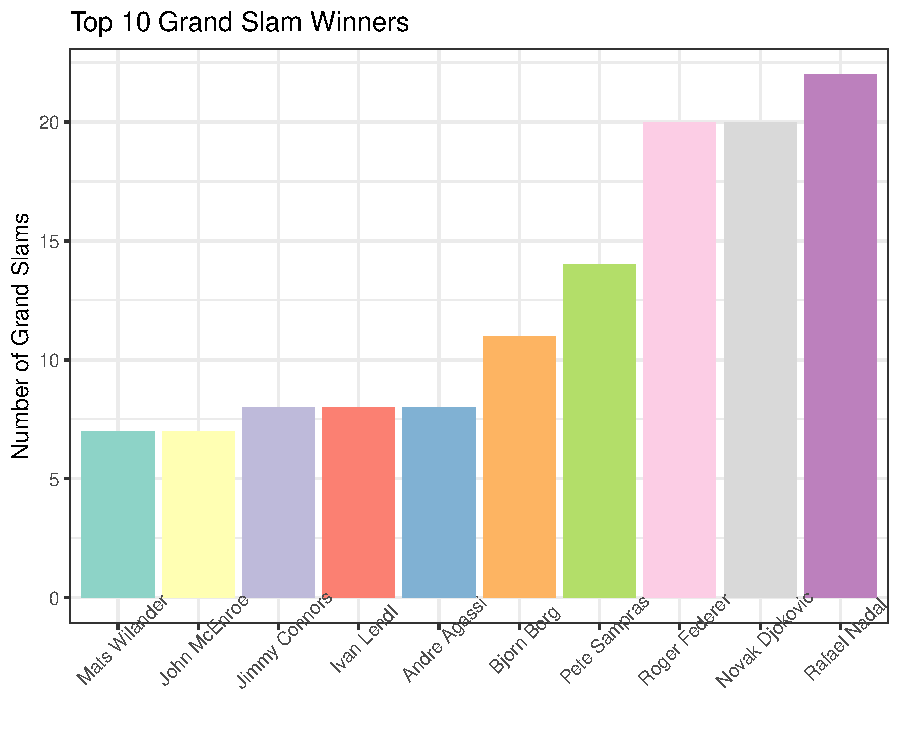
\includegraphics{Write-up_files/figure-latex/GS winners-1.pdf}

This graph illustrates the dominance of the Big 3 in Grand Slam wins,
with Nadal holding the most titles at 22 as of 2022. The other seven
players in the graph, who also had illustrious careers, lag quite far
behind Nadal, Federer and Djokovic. Pete Sampras, for example, who was
still competing when Federer began his career, only has 14 Grand Slams
to his name while the other players have even fewer. This shows how the
Big 3 have elevated the level of the game and raised the bar for what is
considered high-level achievement.

The following table further supports the Big 3's supremacy, showing the
winners of each Grand Slam from 2003 to 2019.

\begin{table}[ht]
\centering
\begin{tabular}{rlllll}
  \hline
 & year & Australian Open & Roland Garros & Wimbledon & US Open \\ 
  \hline
1 & 2003 & Andre Agassi & Juan Carlos Ferrero & Roger Federer & Andy Roddick \\ 
  2 & 2004 & Roger Federer & Gaston Gaudio & Roger Federer & Roger Federer \\ 
  3 & 2005 & Marat Safin & Rafael Nadal & Roger Federer & Roger Federer \\ 
  4 & 2006 & Roger Federer & Rafael Nadal & Roger Federer & Roger Federer \\ 
  5 & 2007 & Roger Federer & Rafael Nadal & Roger Federer & Roger Federer \\ 
  6 & 2008 & Novak Djokovic & Rafael Nadal & Rafael Nadal & Roger Federer \\ 
  7 & 2009 & Rafael Nadal & Roger Federer & Roger Federer & Juan Martin del Potro \\ 
  8 & 2010 & Roger Federer & Rafael Nadal & Rafael Nadal & Rafael Nadal \\ 
  9 & 2011 & Novak Djokovic & Rafael Nadal & Novak Djokovic & Novak Djokovic \\ 
  10 & 2012 & Novak Djokovic & Rafael Nadal & Roger Federer & Andy Murray \\ 
  11 & 2013 & Novak Djokovic & Rafael Nadal & Andy Murray & Rafael Nadal \\ 
  12 & 2014 & Stan Wawrinka & Rafael Nadal & Novak Djokovic & Marin Cilic \\ 
  13 & 2015 & Novak Djokovic & Stan Wawrinka & Novak Djokovic & Novak Djokovic \\ 
  14 & 2016 & Novak Djokovic & Novak Djokovic & Andy Murray & Stan Wawrinka \\ 
  15 & 2017 & Roger Federer & Rafael Nadal & Roger Federer & Rafael Nadal \\ 
  16 & 2018 & Roger Federer & Rafael Nadal & Novak Djokovic & Novak Djokovic \\ 
  17 & 2019 & Novak Djokovic & Rafael Nadal & Novak Djokovic & Rafael Nadal \\ 
   \hline
\end{tabular}
\caption{Grand Slam Winners Since 2003} 
\end{table}

This is evidence of the extent to which Nadal, Federer and Djokovic have
dominated the Grand Slam circuit. Since 2003, when Federer won his first
Grand Slam, the Big 3 have won 55 out of the 68 tournaments in this
period, with only only Andy Murray and Stan Wawrinka winning more than
one each of all the other players. There is therefore no doubt that
these top 3 players will rival each other as being the greatest of all
time. Beyond showing Grand Slam wins, the data also provides additional
information on the statistics of each match played relating to length of
the game, serving and break points statistics and the surface of the
tournament among others. The following tables and figures illustrate how
each of the Big 3's wins are broken down and relate to some of these
variables.

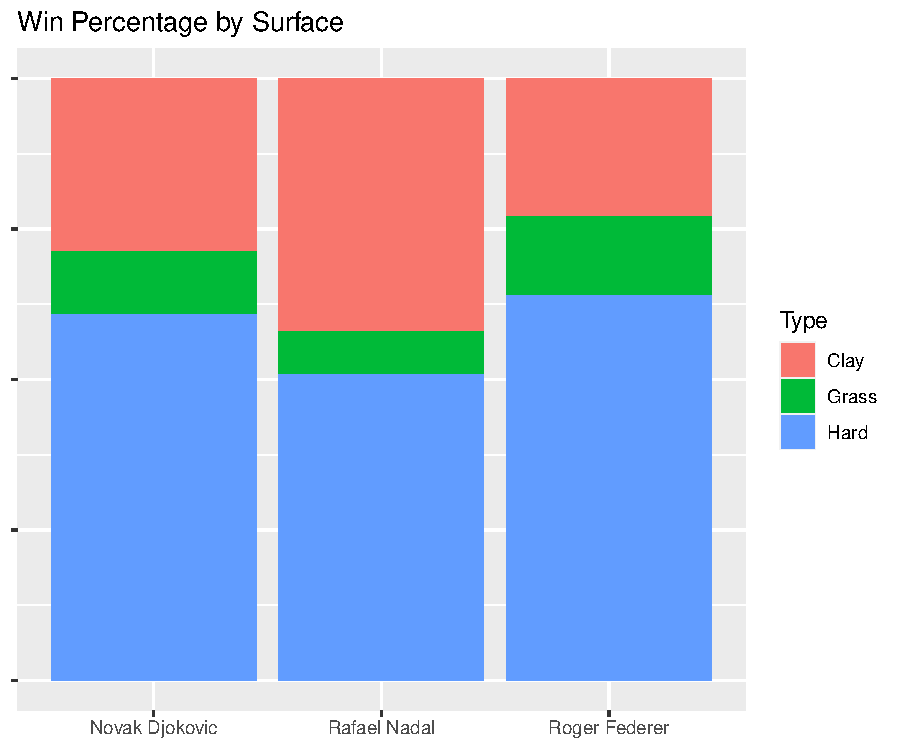
\includegraphics{Write-up_files/figure-latex/more descriptive-1.pdf}

These graphs, referencing surfaces by their colour, show each of Nadal,
Federer and Djokovic's win percentages on each surface. This indicates
that Nadal has a much higher win record on clay than the other two,
confirming his status as the King of Clay. All players have the highest
win records on hard court, which may partly link to this being the
surface with the most number of matches, but Federer and Djokovic have a
more even split across surfaces, indicating their versatility.

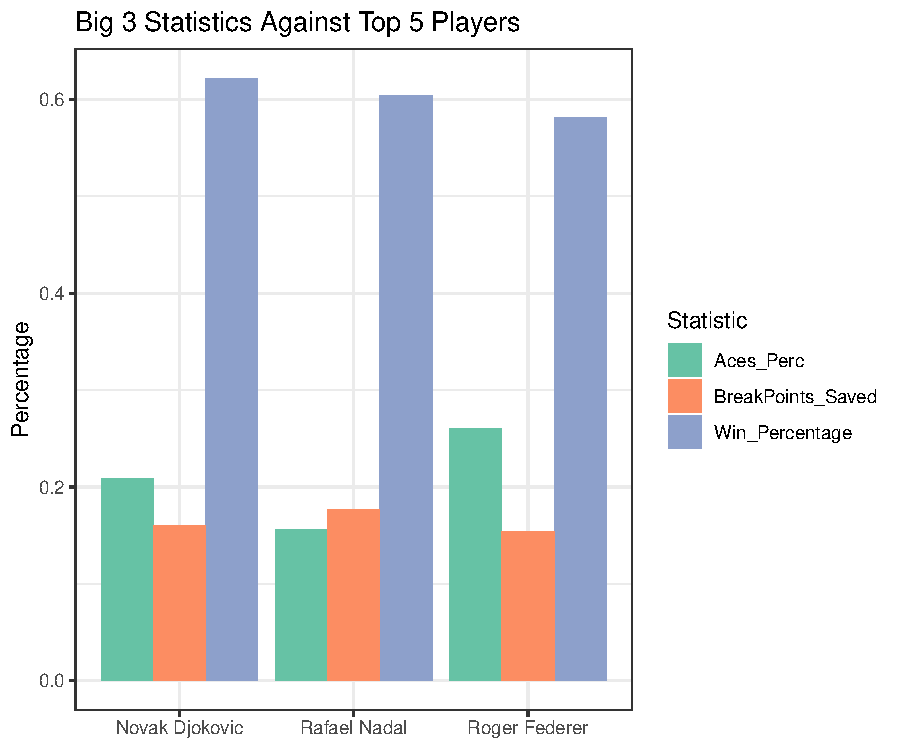
\includegraphics{Write-up_files/figure-latex/grouped bar-1.pdf}

The grouped chart sheds further light into each of the Big 3's
statistics against top 5 players, averaging across matches. Djokovic has
the highest win percentage, Nadal the highest breakpoints saved and
Federer the highest ace percentage. Federer is known to have a strong
serve that is difficult to read so it is understandable that his ace
percentage is higher than the others, while Nadal is known to fight back
when he is at a disadvantage, hence the high breakpoints saved. However,
I would argue that win percentage is the most important statistic to
consider because this relates directly to number of wins and titles.
This graph shows that Djokovic has the best record against top 5 players
in the main ATP events, winning approximately 62 percent of his matches.

\begin{table}[ht]
\centering
\begin{tabular}{rlr}
  \hline
 & Player & TTaken \\ 
  \hline
1 & Rafael Nadal & 125.00 \\ 
  2 & Roger Federer & 109.00 \\ 
  3 & Novak Djokovic & 121.00 \\ 
   \hline
\end{tabular}
\caption{Average Time Taken} 
\end{table}

This final table provides an overview of the Big 3's average match times
across all games. Roger Federer is shown to take the least amount of
time to finish matches, averaging at 109 minutes or approximately 1 hour
and 45 minutes. This is quite significantly different from Nadal and
Djokovic, suggesting that Federer prefers a shorter game format. This
may link to his playing style which involves big serves and net play
which generally induces shorter matches due to less rallies.

These graphs and tables provide a sufficient overview of player
performance and offers a comparison of the Big 3'\,'s results and more
specifics of their playing style and outcomes. However, to obtain a more
definitive answer to the question of the GOAT, I make use of a random
forest model which is discussed and interpreted in the next sections.

\hypertarget{data-and-methodology}{%
\section{Data and methodology}\label{data-and-methodology}}

I have made use of a dataset that includes all the ATP matches from 1968
to 2022, within which is included match and player statistics. I merged
these documents and filtered the data frame to include only main tour
events i.e.~Grand Slams, Masters and Tour Finals. These are the most
important events in the tennis circuit and the ones in which the top
players participate the most. I further subset the data to include
matches from 2003, when Roger Federer won his first Grand Slam at
Wimbledon. This allows me to focus on the time period of the Big 3 who
are at the centre of the debate surrounding the GOAT. There is also a
large amount of missing information in earlier dates, particularly in
the 1960s, 70s and 80s, so subsetting to start at 2003 avoids issues
related to NA values. Finally, I selected the features I deemed most
relevant to my model to arrive at the final data frame.

\hypertarget{the-random-forest-model}{%
\subsection{The random forest model}\label{the-random-forest-model}}

Why I chose a random forest - reference textbook here.

\hypertarget{target-and-feature-engineering}{%
\subsubsection{Target and feature
engineering}\label{target-and-feature-engineering}}

bimodal distribution, factors

\hypertarget{hyperparameter-tuning}{%
\subsubsection{Hyperparameter tuning}\label{hyperparameter-tuning}}

\hypertarget{results-and-discussion}{%
\section{Results and discussion}\label{results-and-discussion}}

\bibliography{Tex/ref}





\end{document}
